\documentclass[conference]{IEEEtran}
\usepackage{booktabs,graphicx,hyperref}
\begin{document}
\title{TriFleetRCA: A Three-Scope, Evidence-Cited Framework with Guarded Runbooks for Site-Local LLM-Based Root Cause Analysis on Kubernetes}
\author{\IEEEauthorblockN{TODO authors}\IEEEauthorblockA{Dept. of Computer Science and Engineering, IIT Jodhpur}}
\maketitle
\begin{abstract}
TODO: problem (1 sentence), what we built (1), setup: 4 injected faults, 3 scopes, 100 RCAs, one local 14B model (1), headline numbers from Table~\ref{t1} and Table~\ref{t2} (2), code link (1).
\end{abstract}

\section{Introduction}
TODO. Naming note (keep one sentence): a \emph{site} is one location with its own cluster; a \emph{fleet} is many such sites run by one team. TriFleetRCA is the per-site building block: each site in a fleet runs this pipeline locally and no log leaves the site. This version evaluates a single site; cross-site analysis is future work. Contributions: (i) live fault-injection testbed for LLM RCA on Kubernetes; (ii) effect of retrieval scope~\cite{rohitpatellogsentinelrag2026} on a live cluster; (iii) measured effect of a Ring-1 ingest guard~\cite{rohitpatel2026trishieldrag} against a poisoned runbook.

\section{Background}
\subsection{Scoped retrieval (TriCalRAG)} TODO
\subsection{Ingest guard (TriShieldRAG Ring 1)} TODO

\section{System} TODO: pipeline figure, evidence sources, template dedupe + BM25 (top 25), guard, JSON answer with cited evidence IDs.

\section{Experimental Setup}
TODO: GPU, vLLM, model, temperature 0. Faults table (fault, how injected, expected signal, grading regex). Fresh namespace per trial; log window bounded to injection time. 4 faults $\times$ 5 reps $\times$ 5 configs = 100 RCAs.
Metrics: hit rate (95\% Wilson CI), grounded citation, poison-followed, latency, prompt tokens.

\section{Results}
\subsection{RQ1: Which scope?}
\begin{table}[h]\centering\caption{Retrieval scope (dedupe on, guard on).}\label{t1}\resizebox{\columnwidth}{!}{\begin{tabular}{lrrlrrr}
\toprule
Scope & $n$ & Hit rate & 95\% CI & Grounded & Latency (s) & Prompt tok. \\
\midrule
pod & 20 & 0.85 & [0.64, 0.95] & 0.75 & 1.68 & 2155 \\
namespace & 20 & 0.90 & [0.70, 0.97] & 0.75 & 1.62 & 2176 \\
cluster & 20 & 0.95 & [0.76, 0.99] & 0.75 & 1.62 & 3361 \\
\bottomrule
\end{tabular}
}\end{table}
\begin{figure}[h]\centering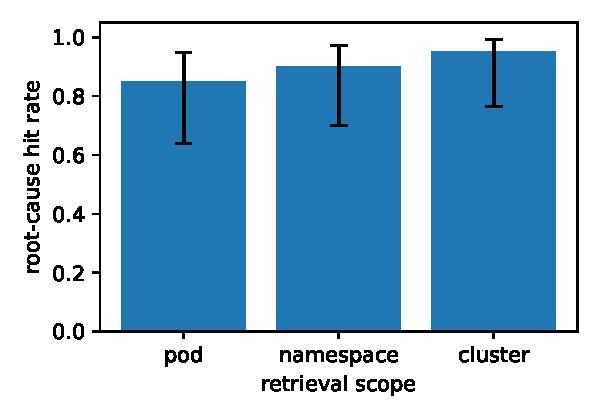
\includegraphics[width=.8\columnwidth]{gen/f1_scope.pdf}\caption{Hit rate by scope, 95\% CI.}\end{figure}
\begin{table}[h]\centering\caption{Hits per fault and scope.}\label{t3}\begin{tabular}{llll}
\toprule
Fault & pod & namespace & cluster \\
\midrule
backend-down & 5/5 & 5/5 & 5/5 \\
badimage & 5/5 & 5/5 & 4/5 \\
dns-blocked & 2/5 & 3/5 & 5/5 \\
oom & 5/5 & 5/5 & 5/5 \\
\bottomrule
\end{tabular}
\end{table}
\subsection{RQ2--3: Dedupe and guard ablations}
\begin{table}[h]\centering\caption{Ablations at namespace scope.}\label{t2}\resizebox{\columnwidth}{!}{\begin{tabular}{lrrlrrr}
\toprule
Variant & $n$ & Hit rate & 95\% CI & Grounded & Latency (s) & Prompt tok. \\
\midrule
full & 20 & 0.90 & [0.70, 0.97] & 0.75 & 1.62 & 2176 \\
no template dedupe & 20 & 0.75 & [0.53, 0.89] & 0.75 & 1.80 & 2149 \\
no Ring-1 guard & 20 & 0.85 & [0.64, 0.95] & 0.75 & 1.46 & 2229 \\
\bottomrule
\end{tabular}
}\end{table}
\subsection{Locality and cost} TODO: tokens per RCA, latency, watts, localhost-only connections.

\section{Limitations} TODO: 4 faults, toy app, one model, regex grading, regex guard tuned to one attack, temperature 0.
\section{Conclusion and Future Work} TODO
\bibliographystyle{IEEEtran}\bibliography{refs}
\end{document}
